\documentclass[conference]{IEEEtran}
\IEEEoverridecommandlockouts
\usepackage{graphicx}
\usepackage{algorithm}
\usepackage{algorithmicx}
\usepackage{algpseudocode}
\usepackage[dvipsnames]{xcolor}
\usepackage{amsmath}
\usepackage{hyperref}

\algblock{Input}{EndInput}
\algnotext{EndInput}
\algblock{Output}{EndOutput}
\algnotext{EndOutput}
\newcommand{\Desc}[2]{\State \makebox[2em][l]{#1}#2}

\newcommand{\tristan}[1]{\color{orange}\textbf{From Tristan:}#1\color{black}}


\begin{document}
\title{I/O simulation model with Linux page cache, integration and evaluation in SimGrid framework}

\author{\IEEEauthorblockN{Hoang-Dung Do, Val\'erie Hayot-Sasson, Tristan Glatard
  }\\
  \IEEEauthorblockA{
    Department of Computer Science and Software Engineering, Concordia University, Montreal, Canada
  }
}

\maketitle

	\begin{abstract}
		\begin{itemize}
			\item The I/O bottleneck in HPC and the need of experiments.
			\item HPC experiment frameworks and advantages of SimGrid.
			\item The missing of the ability to simulate page cache, the goal of this paper.
			\item Principle of the simulator, experiment scenarios and comparisons.
			\item Brief discussion on results and future work.
		\end{itemize}
	\end{abstract}

	\section{Introduction}
		\begin{itemize}
			\item HPC, the bottleneck in I/O and the demand of HPC experiments. 
			\item Difficulties in conducting high performance computing experiments and the need of simulation frameworks.
			\item Existing experiment methods, simulators, simulation frameworks. The advantages of SimGrid compared to others \cite{casanova2008, lebre2015}. The missing of the ability to simulate page cache in SimGrid \cite{lebre2015}.
			\item The objective of the paper: Add capability to simulate I/O with page cache in SimGrid.
		\end{itemize}
	\section{Related Work}			
		
		\subsection{Page cache}
			\begin{itemize}
				\item What is page cache? How it works \cite{linuxdev3rd2010}. Effects and importance of page cache.
				\item Introduce some existing strategies with some highlighted pros and cons.
				\item Current implementation in Linux and some reasons why it is chosen to be implemented (implementation complexity, effectiveness, overhead, etc) \cite{linuxdev3rd2010}
			\end{itemize}									

		\subsection{Simulators}
			\begin{itemize}
				\item Discuss some existing methods, simulation frameworks to conduct HPC experiments. Compare pros and cons (accuracy, simulation time, usability) of some simulators (SimGrid, GridSim).
				\item Related development: RAM energy consumption \cite{gill2019} \cite{ouarnoughi2017} 
				\item Discuss the pros of SimGrid and the reasons why we chose it to extend. (Section 2.2.2 in \cite{casanova2014})
			\end{itemize}
			
	\section{Method}
		In this section, we present our approach to model file read/write, 
		I/O in memory, data flushing and cache eviction mechanisms 
		implemented in Linux. 
		We also detail the design the simulators in order to simulate I/O activities 
		and the implementation in Python and SimGrid framework. 
		Finally, we describe some experimental scenarios to evaluate our model 
		with a Python simulator, a baseline SimGrid simulator, a simulator 
		with SimGrid integrated with our model, and the results from real pipelines.

		\subsection{Principle of the simulator}
	
			In our I/O simulation model, we try to simulate the write back page cache 
			mechanisms including memory I/O, cache eviction and data flushing as we 
			believe that they are the most important factors that affect the I/O time. 

			Memory is modeled with capacity, read bandwidth and write 
			bandwidth. When data is read from or written to memory, the actual 
			read/write time is calculated with the amount of data and memory 
			read/write bandwidth:
			
			\begin{align*}
				& t_{mr} = D / r_m \\ 
				& t_{mw} = D / w_m\
			\end{align*}		
			
			where:
			\begin{itemize}
				\item $t_{mr}$ is time to read data from memory
				\item $t_{mw}$ is time to write data to memory
				\item $D$ is the amount of data to read/write
				\item $r_m$ is memory read bandwidth
				\item $w_m$ is memory write bandwidth
			\end{itemize}						
			
			We introduce the concept of data block as a unit to represent cached data. 
			A data block is a subset of pages of a file in page cache that is accessed 
			at a specific time. Therefore, a block has the information about file name, 
			block size, last access and a dirty flag with values of 0 and 1, 
			0 represents block of lean data, while 1 indicates that the data block 
			is dirty. 
			Cached data of a file can be represented by multiple blocks. 
			Because a data block represents a subset of cached pages, 
			it can be split into smaller blocks, and multiple blocks can also 
			be merged into a larger one.
			
			In Linux kernel, the page cache LRU lists are lists of pages of 
			files in cache. In our simulator, instead of using lists of pages, 
			we simulate these lists with two lists of data blocks, an active list and 
			an inactive list, ordered by block last access as is shown in 
			Figure~\ref{fig:lrulist}.
			As in the kernel, in our simulator, we keep the size of the active list not 
			larger than twice the size of the inactive list by moving least recently 
			used blocks from the active list to the inactive list. 
			
			\begin{figure}
   				\centering
   				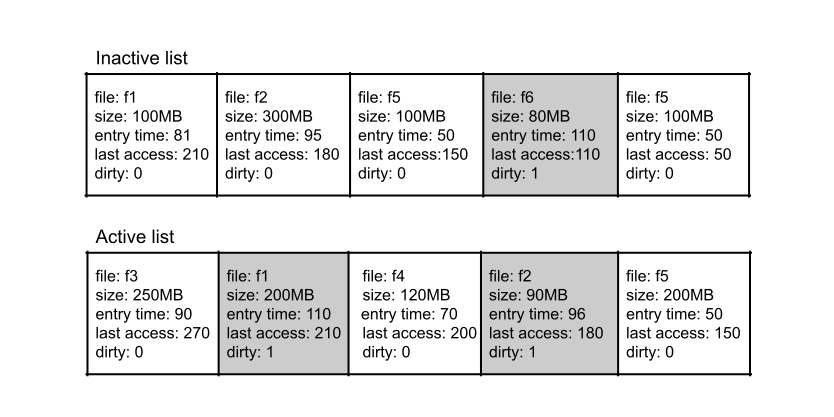
\includegraphics[width=\columnwidth]{figures/lru_lists.pdf}
   				\caption{Simulation of page cache LRU lists with data blocks}\label{fig:lrulist}
			\end{figure}	
			
			Modeling page cache LRU lists as lists of blocks offers our simulator 
			some obvious advantages. 
			Maintaining and handling lists of pages in the simulator, which is in 
			packet level, are non-trivial when they require significant implementation 
			overhead and would likely to hinder the performance of the simulator. 
			Therefore, using page cache lists of data blocks can simplify the 
			simulation of cache eviction and data flushing while preserving
			the accuracy in i/o time simulation. 
			
			With the simulation model of page cache LRU lists of blocks, now we can 
			model I/O in memory.
			At the time when a file is accessed, some data of the file can be in 
			cache or not. 
			If accessed data is already cached, there are existing data blocks 
			representing cached data in two page cache LRU lists. 
			As cached data is accessed again, these blocks are moved to 
			the active list, dirty blocks are merged into a bigger dirty block, 
			while clean data blocks are merged into another clean block. 
			If accessed data is not in cache, new blocks representing uncached data 
			are created and put into the top of the inactive list. 
			For more detail when uncached data is accessed, in the case of 
			reading file, as all uncached data is clean data, only one clean data 
			block is added to the inactive list.
			But in the case of writing uncached file data though cache, 
			this written data can be either dirty or clean. 
			Thus, at most two data blocks can be added to the inactive lists, 
			one is clean and one is dirty. 
			We also keep the size of the active list not larger than twice the size of 
			the inactive list as in the kernel. This is done by moving least recently 
			used blocks in the active list to the inactive list when the active list 
			grows. If only a part of a data block needs to be moved, 
			the block is split.

			Next, we simulate data flushing mechanism, which writes back 
			dirty data to disk. 
			The data flushing simulation function traverses the sorted inactive first, 
			and then the active list, looks for least recently used dirty blocks and 
			sets dirty flags of these blocks to 0 until the total flushed amount 
			reaches the amount to be flushed or there is no dirty data left in cache. 
			If the last flushed block is not entirely flushed, it is split into 
			two blocks, one is flushed and one remains dirty.
			The flushing time is calculated as:
					
			\begin{align*}
				t_f = A / w_d
			\end{align*}		
			
			where:
			\begin{itemize}
				\item $t_f$ is the flushing time
				\item $A$ is the amount of data to be flushed
				\item $w_d$ is the disk write bandwidth
			\end{itemize}		
			
			For periodical flushing, because dirty data can be flushed during CPU time 
			or cache read with disk write bandwidth, the amount of flushed data is 
			calculated with disk bandwidth and flushing duration.
				
			Similarly, our cache eviction simulation function frees up the page cache 
			by traversing and deleting least recently used clean data blocks 
			in the inactive list.
			The amount of evicted data is passed in and data blocks are deleted 
			from the inactive list until total evicted data reaches the amount 
			passed in, or there is no clean block left in the list.
			If the last evicted block is not entirely evicted, the block is split, 
			and only one block is deleted.
			Our cache eviction simulation does not add up to the simulated time 
			since cache eviction time is negligible in real systems.			
			
			We encapsulate the models of memory and page cache LRU lists in 
			\textit{MemoryManager} class. 
			The functionalities of this class are exposed to the simulation  
			of I/O activities including file read and file write. 
			We create \textit{IOController} class which simulates file read and 
			file write by interacting with the MemoryManager class, 
			exposing APIs to user simulated applications. 
			These two class act as an extra layer with kernel-like functionalities as 
			illustrated in Figure~\ref{fig:interaction}. 
			Simulated applications can simply request for a file read 
			or file write by calling the APIs of this layer instead of 
			calling directly to storage simulation models.
			Because every computer has its own memory and system configurations, 
			one IOController object and one MemoryManager object are created 
			for each simulated machine.
			
			\begin{figure}
   				\centering
   				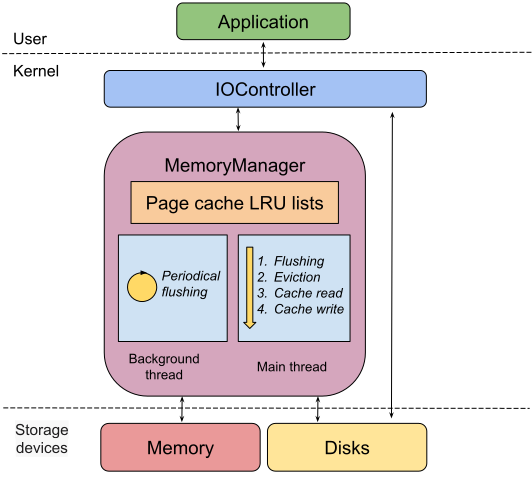
\includegraphics[width=0.85\columnwidth]{figures/interaction.pdf}
   				\caption{The additional layer between user application layer and 
   				storage simulation models}\label{fig:interaction}
			\end{figure}				

			To read or write a file, a simulated application sends a request to the 
			IOController instance on the node where the requested file is stored.
			Based on the memory status in MemoryManager, the IOController 
			orchestrates cache read/write, disk read/write, flushing and cache eviction 
			to fulfill I/O requests, calculates total simulated time and returns to 
			simulated applications.
			
			\begin{algorithm}\caption{File read simulation}\label{alg:read}
				\small
				\begin{algorithmic}[1]
					\Input
        				\Desc{fn}{file name}
        				\Desc{fs}{file size (assumed to fit in memory)}
						\Desc{rt}{current simulated run time}
						\Desc{mm}{MemoryManager object}
						\Desc{$r_m$}{memory read bandwidth}
						\Desc{$r_d$}{disk read bandwidth}
   					\EndInput
   					\Output
						\Desc{rt}{simulated run time after the file is read}
   					\EndOutput
					\State rt = rt + mm.flush(2*fs - mm.cached(fn) - mm.avail\_mem)
					\State mm.evict(2*fs - mm.cached(fn) - mm.free\_mem) 
					\If {mm.cached(fn) $>$ 0}  \Comment{Read file cached data}
    					\State mm.cache\_read(fn) 
						\State rt = rt + mm.cached(fn) / $r_m$
					\EndIf
					\If {mm.cached(fn) $<$ fs} \Comment{Read uncached data from disk}
						\State mm.disk\_read(fs - mm.cached(fn), fn)
    					\State rt = rt + (fs - mm.cached(fn)) / $r_d$
					\EndIf					
					
					\State \Return rt
					
				\end{algorithmic}
			\end{algorithm}			
			
			The algorithm used to simulate file read is described in 
			Algorithm~\ref{alg:read}. 
			In Linux systems with write back storage devices, data can be either read 
			from cache with memory bandwidth or read from disk with disk bandwidth. 
			Therefore, total read time can be considered as a linear function 
			of the read time with each of these bandwidths, 
			enabling us to generalize reading process as two separate phases, 
			cache read and disk read. 
			In our simulator, when a user simulated application reads a file, 
			it sends a file read request to IOController. 
			Then, IOController calculates the amount of required memory to read 
			the file based on the amount of available memory, file size, and 
			the amount of cached data of that file (line 10). 
			If there is not enough available memory, dirty data is flushed to disk 
			to increase the amount of memory available by calling flush function 
			of MemoryManager with the amount of flushed data, flushing time is 
			simulated and added to total run time (line 11-12).
			After data is flushed, MemoryManager is asked to evict data 
			from cache to accommodate the requested file (line 13-14). 
			Next, if file is cached either partially or entirely, MemoryManager is 
			called to re-access and update this cached data (line 16). 
			If all file data is cached, periodical flushing is called is to flush 
			dirty data during the cache read, and time to read from cache is added to 
			total run time, (line 18-20). 
			If file is not cached or partially cached, a disk read is required (line 23) 
			This blocks flushing and makes the cache read time neglectable. 
			Finally, data is read from disk to cache and managed 
			by MemoryManager, disk read time is estimated with disk read 
			bandwidth and added to total run time (line 24-25). 

			\begin{algorithm}\caption{File write simulation}\label{alg:write}
				\small
				\begin{algorithmic}[1]
					\Input
        				\Desc{fn}{file name}
        				\Desc{fs}{file size}
						\Desc{rt}{current simulated run time}
						\Desc{mm}{MemoryManager object}
						\Desc{$w_m$}{memory write bandwidth}
						\Desc{$w_d$}{disk write bandwidth}
   					\EndInput
   					\Output
						\Desc{rt}{simulated run time after the file is read}
   					\EndOutput
					\State dirty\_left = $d$ * mm.avail\_mem - mm.dirty
					\If {dirty\_left $>$ 0}
   						\State free\_amt = min(fs, $M$) \Comment{$M$ in Equation
   						~\ref{equa:freeamt}}
    					\State mm.evict(free\_amt - mm.free\_mem)
    					\State free\_time = free\_amt / $w_m$
    					\State mm.write(fn, free\_amt, dirty = free\_amt - free\_time * $w_d$)
   						\State rt = rt + free\_time
    				\EndIf
					
					\If {free\_amt $\geq$ fs}
						\Return rt
					\EndIf

					\State throttled\_amt = fs - free\_amt \Comment{Written with disk bandwidth}
					\State req = max(0, throttled\_amt  - mm.free\_mem)
					\State evicted\_amt = min(req, mm.evictable)
					\State mm.evict(evicted\_amt)
					\State cached\_amt = min(mm.free\_mem, throttled\_amt)
					\State mm.write(fn, cached = cached\_amt, dirty = 0)
					\State rt = rt + throttled\_amt /$w_d$

					\Return rt
					
				\end{algorithmic}
			\end{algorithm}

			Algorithm~\ref{alg:write} describes our simulation of file write. 
			Similar to the file read simulation, a file can also be written with 
			two different bandwidths, memory bandwidth and disk bandwidth. 
			Files can be written with memory bandwidth before the amount 
			of dirty data reaches dirty\_ratio. Thus, our algorithm initially checks 
			this condition (line 10), and estimates the maximum amount 
			of data can be written with memory bandwidth with the following 
			formula:
			
			\begin{equation}
				M = max(0, \frac{(d*C - D)*w_m}{w_m - w_d})\label{equa:freeamt}
			\end{equation}			 			

			where:
			\begin{itemize}
				\item $M$ is the maximum amount of data that can be written with memory 
				write bandwidth
				\item $d$ is dirty ratio
				\item $C$ is the total available memory
				\item $D$ is the amount of dirty data
				\item $w_m$ is the memory write bandwidth 
				\item $w_d$ is the disk write bandwidth			
			\end{itemize}
			
			In this formula, we assume that data is written with with memory 
			bandwidth until dirty\_ratio is reached, the kernel writes data 
			to cache and flushes dirty data to disk concurrently. 
			If file size is smaller than or equal to $M$, the whole file is 
			written to cache as dirty data with memory bandwidth (line 12). 
			Otherwise, the remaining file data is written with disk bandwidth (line 20). 
			Before simulating cache write, MemoryManager is asked to evict 
			the page cache to accommodate written data (line 13). 
			Then, data is written to cache as dirty data with memory 
			bandwidth, and write time is added to total simulated time (line 14-16). 
			Because cache write and data flushing are concurrent in our algorithm, 
			the actual amount of written dirty data reduces by the amount 
			of data during cache write time (line 15). 
			If not all data is written with memory write bandwidth, the remaining data 
			is written with disk write bandwidth. This can simulate both cases that 
			data is written directly to disk, or applications wait for dirty data 
			to be flushed, and evicted to write new data. 
			If the amount of free memory is not enough for the remaining file data, 
			evictable memory is evicted (line 20-23). 
			Here, the simulator does not guarantee that the amount of free memory 
			after eviction can accommodate the remaining data. 
			In the case that free memory is less than remaining data, the amount to be 
			cached is limited by the amount of free memory (line 24). 
			However, the kernel still flushes, evicts and writes new data concurrently, 
			and remaining data is still written to cache with disk write bandwidth.
			Thus, we can simulate the time to write the remaining data with 
			disk bandwidth and ask MemoryManager to add clean cached data (line 25). 
			The simulated time to write width disk bandwidth is added to total 
			simulated run time and returned to simulated applications (line 26).	
			
		\subsection{Implementation}

			To validate our simulation model, we create a simple 
			simulator which is independent to simulation frameworks and libraries. 
			This enables us to evaluate the accuracy and correctness of our 
			model in a simple use case before integrating it to SimGrid. 
			This simulator simulates a single-threaded pipeline running on a system 
			with a single core CPU, one local storage device and all input and 
			output files are stored locally. The results from the simulator is compared 
			and validated with the results from a real pipeline running on
			a real system.
			
			Having our model validated, we create simulators for different use cases 
			using the current version of SimGrid and the SimGrid version that is 
			extended with our model. We leverage Wrench framework, which is 
			built on top of SimGrid to simulate our pipelines and system.
			Then, we compare the results of the simulators with
			original SimGrid and extended SimGrid with the results of real
			pipelines on a real system. 
		
			In this work, we use Python 3.7 to implement the simple
			simulator, SimGrid 3.25 and Wrench 1.6 for SimGrid simulators. 
			SimGrid source code is available at 
			\url{https://framagit.org/simgrid/simgrid}, and Wrench is provided on
			github at \url{https://github.com/wrench-project/wrench}.
			
		\subsection{Experiments}
		
			When designing experiments, our goal is to evaluate our simulation model 
			in single-threaded and multi-threaded applications which access data on 
			on different file system types. 
			To do that, we create a pipeline of sequential tasks, each task 
			reads an input file, increases every byte of the input, and writes the 
			output to disk. The output of the previous task is the input of 
			the next task. We also adopt an use case in real applications and 
			to evaluate the applicability of our simulation model.
			
			The simplest scenario is a single-threaded application, where memory 
			bandwidth and disk bandwidth are not shared with another thread. 
			This allows us to compare the detailed results in terms of read/write time, 
			memory states after every single task and ,more importantly, validate our 
			simulation model. 
			
			For multi-threaded applications, we do the experiment with a varying 
			number of concurrent pipelines running on a multi-core host 
			and writing to the same local storage device. 
		    By doing so, we can assess the performance of our model in the case  
		    of concurrent I/O with shared bandwidth on a local storage device.
		    
		    Since different storage types should also be taken into account, 
		    we conduct the next experiment with the same scenario as 
		    in the multi-threaded experiment, except that files are stored on a 
		    shared file system instead of local disk. 
		    In this way, we can not only evaluate our simulation model on I/O 
		    with shared file system, but also compare the 
		    performance of the simulator on different storage types. 
		    
		    Finally, we adopt a real pipeline in a real neuroimaging applications. 
		    We simulate the pipeline with a simulated workflow in SimGrid 
			and compare the simulation results with the real results. 
			Because our work focuses on I/O time, we assume that CPU time is 
			correctly modeled and use the CPU time measured in the real pipelines 
			to setup our simulated workflows. 
			
			We use the cluster of \textit{Big Data Infrastructure for Neuroimaging Lab} 
			at \textit{Concordia University} to conduct our experiments. The cluster 
			consists of one login node which is the control node, 8 compute nodes 
			and 4 storage nodes connected with two network switches. The login node 
			has one Intel(R) Xeon(R) Gold 6130 CPU @ 2.10GHz, 128GiB of RAM, 1.8TB 
			of storage of XFS file system, 13GB of tmpfs file system and 385 TB of 
			Lustre shared file system. Each compute node has two 16 cores Intel(R) 
			Xeon(R) Gold 6130 CPU @ 2.10GHz, 256 GB of RAM and 6 SSDs, 450GB each 
			with XFS file system, 378GB of tmpfs and 126GB of devtmpfs file system.
			Lustre file system is configured with one metadata target with 854GB 
			of storage, 44 object storage targets with 8.7TB of storage each. 
			The cluster is run on CentOS 8.1 with the Slurm Workload Manager installed. We use 
			\textbf{\textit{atop}} and \textbf{\textit{collectl}} as tools to monitor 
			and collect data of memory, page cache status and disk throughput on 
			the cluster. The cluster nodes are connected with ... 
			\textcolor{red}{[network description here]}
	
			\subsubsection{Single-threaded evaluation}

				In this experiment, our goal is to validate our model by comparing 
				the simulation results of the simple Python simulator with results of 
				a simulator implemented with original SimGrid, a simulator 
				implemented with SimGrid integrated with our model, and a real pipeline 
				running of the cluster. 
				The pipeline consists of three tasks, each task reads a file, 
				increases every byte and writes output file to local disk. 
				We use the input sizes of 20 GB, 50 GB, 75 GB and 100 GB, run 
				the pipeline on the cluster, measure the CPU time of the pipeline 
				with each input to simulate the pipeline with the simulators.

			\subsubsection{Multi-threaded evaluation}

				In the second experiment, we evaluate the simulator in concurrent I/O 
				with a multi-threaded application. As we run the pipelines on 
				only one compute node of the cluster, which has upto 32 cores per node,  
				we create 32 input files with the size of 3GB each and vary the number of 
				concurrent pipelines from 1 to 32. 
				Because multi-threaded simulator implementation in Python is 
				expensive, and we have our model integrated in SimGrid, 
				we only compare the results of simulators with original SimGrid, 
				SimGrid integrated with our model and and real pipelines. 
				The results are compared in total makespan of the pipelines, 
				cumulative read time and cumulative write time.
			
			\subsubsection{Evaluation on storage types}

				

			\subsubsection{Simulation of a real application}
				A real pipeline (for example a pipeline with nighres)

	\section{Results}
	
		\begin{itemize}

			\item Quantitative results: 
				\begin{itemize}
					\item Errors of simulation time and memory used compared to real results.
					\item Simulation time compared to baseline SimGrid.
				\end{itemize} 

			\item Ability of the model to generalize memory trends (dirty data, cache used) and disk throughput.

		\end{itemize}

	\section{Discussion and Future Work}
		\begin{itemize}
			\item Sensitivity of the simulator on the variation of memory and disk bandwidth. 
		\end{itemize}
\bibliographystyle{plain}
\bibliography{citation}

\end{document}